\documentclass[11pt,letter]{article}
\usepackage{amsmath,amsthm,amssymb,hyperref,verbatim}
\usepackage{tikz}
\usetikzlibrary{shapes.geometric,decorations.pathreplacing,calligraphy,patterns,patterns.meta}

\newcommand{\cohort}{\mathcal{C}}

\begin{document}

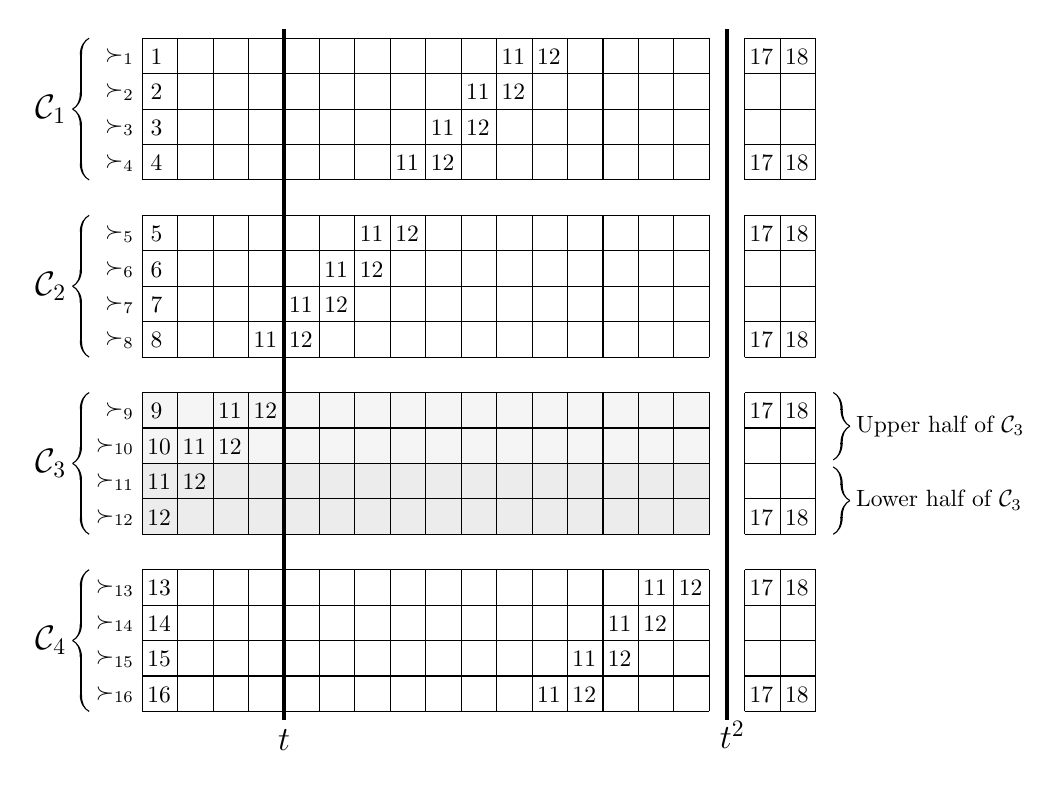
\begin{tikzpicture}
\begin{scope}[scale=0.45,every node/.style={align=center,scale=0.85}]
    % cohorts
    \draw (0, 0) grid (16,-4);
    \draw (0,-5) grid (16,-9);
    \draw[fill=lightgray!15] (0,-10) grid (16,-12) rectangle (0,-10);
    \draw[fill=lightgray!30] (0,-12) grid (16,-14) rectangle (0,-12);
    \draw (0,-15) grid (16,-19);
    % Cohort 1
    \draw [decorate,decoration={calligraphic brace,amplitude=6pt},thick] (-1.5,-4) -- (-1.5,0) node[left=6pt,pos=.5]{\Large $\cohort_1$};
    \draw (0,-1) node[left,yshift=.25cm]{$\succ_1$};
    \draw (0,-2) node[left,yshift=.25cm]{$\succ_2$};
    \draw (0,-3) node[left,yshift=.25cm]{$\succ_3$};
    \draw (0,-4) node[left,yshift=.25cm]{$\succ_4$};
    \draw (0,-1) node[right,yshift=.25cm]{1};
    \draw (10,-1) node[right,yshift=.25cm,xshift=-.05cm]{11};
    \draw (11,-1) node[right,yshift=.25cm,xshift=-.05cm]{12};
    \draw (0,-2) node[right,yshift=.25cm]{2};
    \draw (9,-2) node[right,yshift=.25cm,xshift=-.05cm]{11};
    \draw (10,-2) node[right,yshift=.25cm,xshift=-.05cm]{12};
    \draw (0,-3) node[right,yshift=.25cm]{3};
    \draw (8,-3) node[right,yshift=.25cm,xshift=-.05cm]{11};
    \draw (9,-3) node[right,yshift=.25cm,xshift=-.05cm]{12};
    \draw (0,-4) node[right,yshift=.25cm]{4};
    \draw (7,-4) node[right,yshift=.25cm,xshift=-.05cm]{11};
    \draw (8,-4) node[right,yshift=.25cm,xshift=-.05cm]{12};
     % Cohort 2
     \draw [decorate,decoration={calligraphic brace,amplitude=6pt},thick] (-1.5,-9) -- (-1.5,-5) node[left=6pt,pos=.5]{\Large $\cohort_2$};
    \draw (0,-6) node[left,yshift=.25cm]{$\succ_5$};
    \draw (0,-7) node[left,yshift=.25cm]{$\succ_6$};
    \draw (0,-8) node[left,yshift=.25cm]{$\succ_7$};
    \draw (0,-9) node[left,yshift=.25cm]{$\succ_8$};
    \draw (0,-6) node[right,yshift=.25cm]{5};
    \draw (6,-6) node[right,yshift=.25cm,xshift=-.05cm]{11};
    \draw (7,-6) node[right,yshift=.25cm,xshift=-.05cm]{12};
    \draw (0,-7) node[right,yshift=.25cm]{6};
    \draw (5,-7) node[right,yshift=.25cm,xshift=-.05cm]{11};
    \draw (6,-7) node[right,yshift=.25cm,xshift=-.05cm]{12};
    \draw (0,-8) node[right,yshift=.25cm]{7};
    \draw (4,-8) node[right,yshift=.25cm,xshift=-.05cm]{11};
    \draw (5,-8) node[right,yshift=.25cm,xshift=-.05cm]{12};
    \draw (0,-9) node[right,yshift=.25cm]{8};
    \draw (3,-9) node[right,yshift=.25cm,xshift=-.05cm]{11};
    \draw (4,-9) node[right,yshift=.25cm,xshift=-.05cm]{12};
    % Cohort 3
    \draw [decorate,decoration={calligraphic brace,amplitude=6pt},thick] (-1.5,-14) -- (-1.5,-10) node[left=6pt,pos=.5]{\Large $\cohort_3$};
    \draw [decorate,decoration={calligraphic brace,amplitude=6pt},thick] (19.5,-10) -- (19.5,-11.9) node[right=6pt,pos=.5]{Upper half of $\cohort_3$};
    \draw [decorate,decoration={calligraphic brace,amplitude=6pt},thick] (19.5,-12.1) -- (19.5,-14) node[right=6pt,pos=.5]{Lower half of $\cohort_3$};
    \draw (0,-11) node[left,yshift=.25cm]{$\succ_9$};
    \draw (0,-12) node[left,yshift=.25cm]{$\succ_{10}$};
    \draw (0,-13) node[left,yshift=.25cm]{$\succ_{11}$};
    \draw (0,-14) node[left,yshift=.25cm]{$\succ_{12}$};
    \draw (0,-11) node[right,yshift=.25cm]{9};
    \draw (2,-11) node[right,yshift=.25cm,xshift=-.05cm]{11};
    \draw (3,-11) node[right,yshift=.25cm,xshift=-.05cm]{12};
    \draw (0,-12) node[right,yshift=.25cm,xshift=-.05cm]{10};
    \draw (1,-12) node[right,yshift=.25cm,xshift=-.05cm]{11};
    \draw (2,-12) node[right,yshift=.25cm,xshift=-.05cm]{12};
    \draw (0,-13) node[right,yshift=.25cm,xshift=-.05cm]{11};
    \draw (1,-13) node[right,yshift=.25cm,xshift=-.05cm]{12};
    \draw (0,-14) node[right,yshift=.25cm,xshift=-.05cm]{12};
    % Cohort 4
    \draw [decorate,decoration={calligraphic brace,amplitude=6pt},thick] (-1.5,-19) -- (-1.5,-15) node[left=6pt,pos=.5]{\Large $\cohort_4$};
    \draw (0,-16) node[left,yshift=.25cm]{$\succ_{13}$};
    \draw (0,-17) node[left,yshift=.25cm]{$\succ_{14}$};
    \draw (0,-18) node[left,yshift=.25cm]{$\succ_{15}$};
    \draw (0,-19) node[left,yshift=.25cm]{$\succ_{16}$};
    \draw (0,-16) node[right,yshift=.25cm,xshift=-.05cm]{13};
    \draw (14,-16) node[right,yshift=.25cm,xshift=-.05cm]{11};
    \draw (15,-16) node[right,yshift=.25cm,xshift=-.05cm]{12};
    \draw (0,-17) node[right,yshift=.25cm,xshift=-.05cm]{14};
    \draw (13,-17) node[right,yshift=.25cm,xshift=-.05cm]{11};
    \draw (14,-17) node[right,yshift=.25cm,xshift=-.05cm]{12};
    \draw (0,-18) node[right,yshift=.25cm,xshift=-.05cm]{15};
    \draw (12,-18) node[right,yshift=.25cm,xshift=-.05cm]{11};
    \draw (13,-18) node[right,yshift=.25cm,xshift=-.05cm]{12};
    \draw (0,-19) node[right,yshift=.25cm,xshift=-.05cm]{16};
    \draw (11,-19) node[right,yshift=.25cm,xshift=-.05cm]{11};
    \draw (12,-19) node[right,yshift=.25cm,xshift=-.05cm]{12};
    % Separators
    \draw[very thick] (4,.25) -- (4,-19.25) node[below]{\Large $t$};
    \draw[very thick] (16.5,.25) -- (16.5,-19.25) node[below,yshift=.12cm,xshift=.08cm]{\Large $t^2$};
    % Tail alternatives
    \draw (17, 0) grid (19,-4);
    \draw (17,-1) node[right,yshift=.25cm,xshift=-.05cm]{17};
    \draw (18,-1) node[right,yshift=.25cm,xshift=-.05cm]{18};
    \draw (17,-4) node[right,yshift=.25cm,xshift=-.05cm]{17};
    \draw (18,-4) node[right,yshift=.25cm,xshift=-.05cm]{18};
    \draw (17,-5) grid (19,-9);
    \draw (17,-6) node[right,yshift=.25cm,xshift=-.05cm]{17};
    \draw (18,-6) node[right,yshift=.25cm,xshift=-.05cm]{18};
    \draw (17,-9) node[right,yshift=.25cm,xshift=-.05cm]{17};
    \draw (18,-9) node[right,yshift=.25cm,xshift=-.05cm]{18};
    \draw (17,-10) grid (19,-14);
    \draw (17,-11) node[right,yshift=.25cm,xshift=-.05cm]{17};
    \draw (18,-11) node[right,yshift=.25cm,xshift=-.05cm]{18};
    \draw (17,-14) node[right,yshift=.25cm,xshift=-.05cm]{17};
    \draw (18,-14) node[right,yshift=.25cm,xshift=-.05cm]{18};
    \draw (17,-15) grid (19,-19);
    \draw (17,-16) node[right,yshift=.25cm,xshift=-.05cm]{17};
    \draw (18,-16) node[right,yshift=.25cm,xshift=-.05cm]{18};
    \draw (17,-19) node[right,yshift=.25cm,xshift=-.05cm]{17};
    \draw (18,-19) node[right,yshift=.25cm,xshift=-.05cm]{18};
\end{scope}
\end{tikzpicture}

\end{document}